\documentclass[border=10pt]{standalone}

\usepackage{tikz}
\usepackage{tikzsymbols}
\usetikzlibrary{calc,patterns,shapes.geometric}

\def\centerarc[#1](#2)(#3:#4:#5){\draw[#1] ($(#2)+({#5*cos(#3)},{#5*sin(#3)})$) arc (#3:#4:#5);}

\begin{document}
	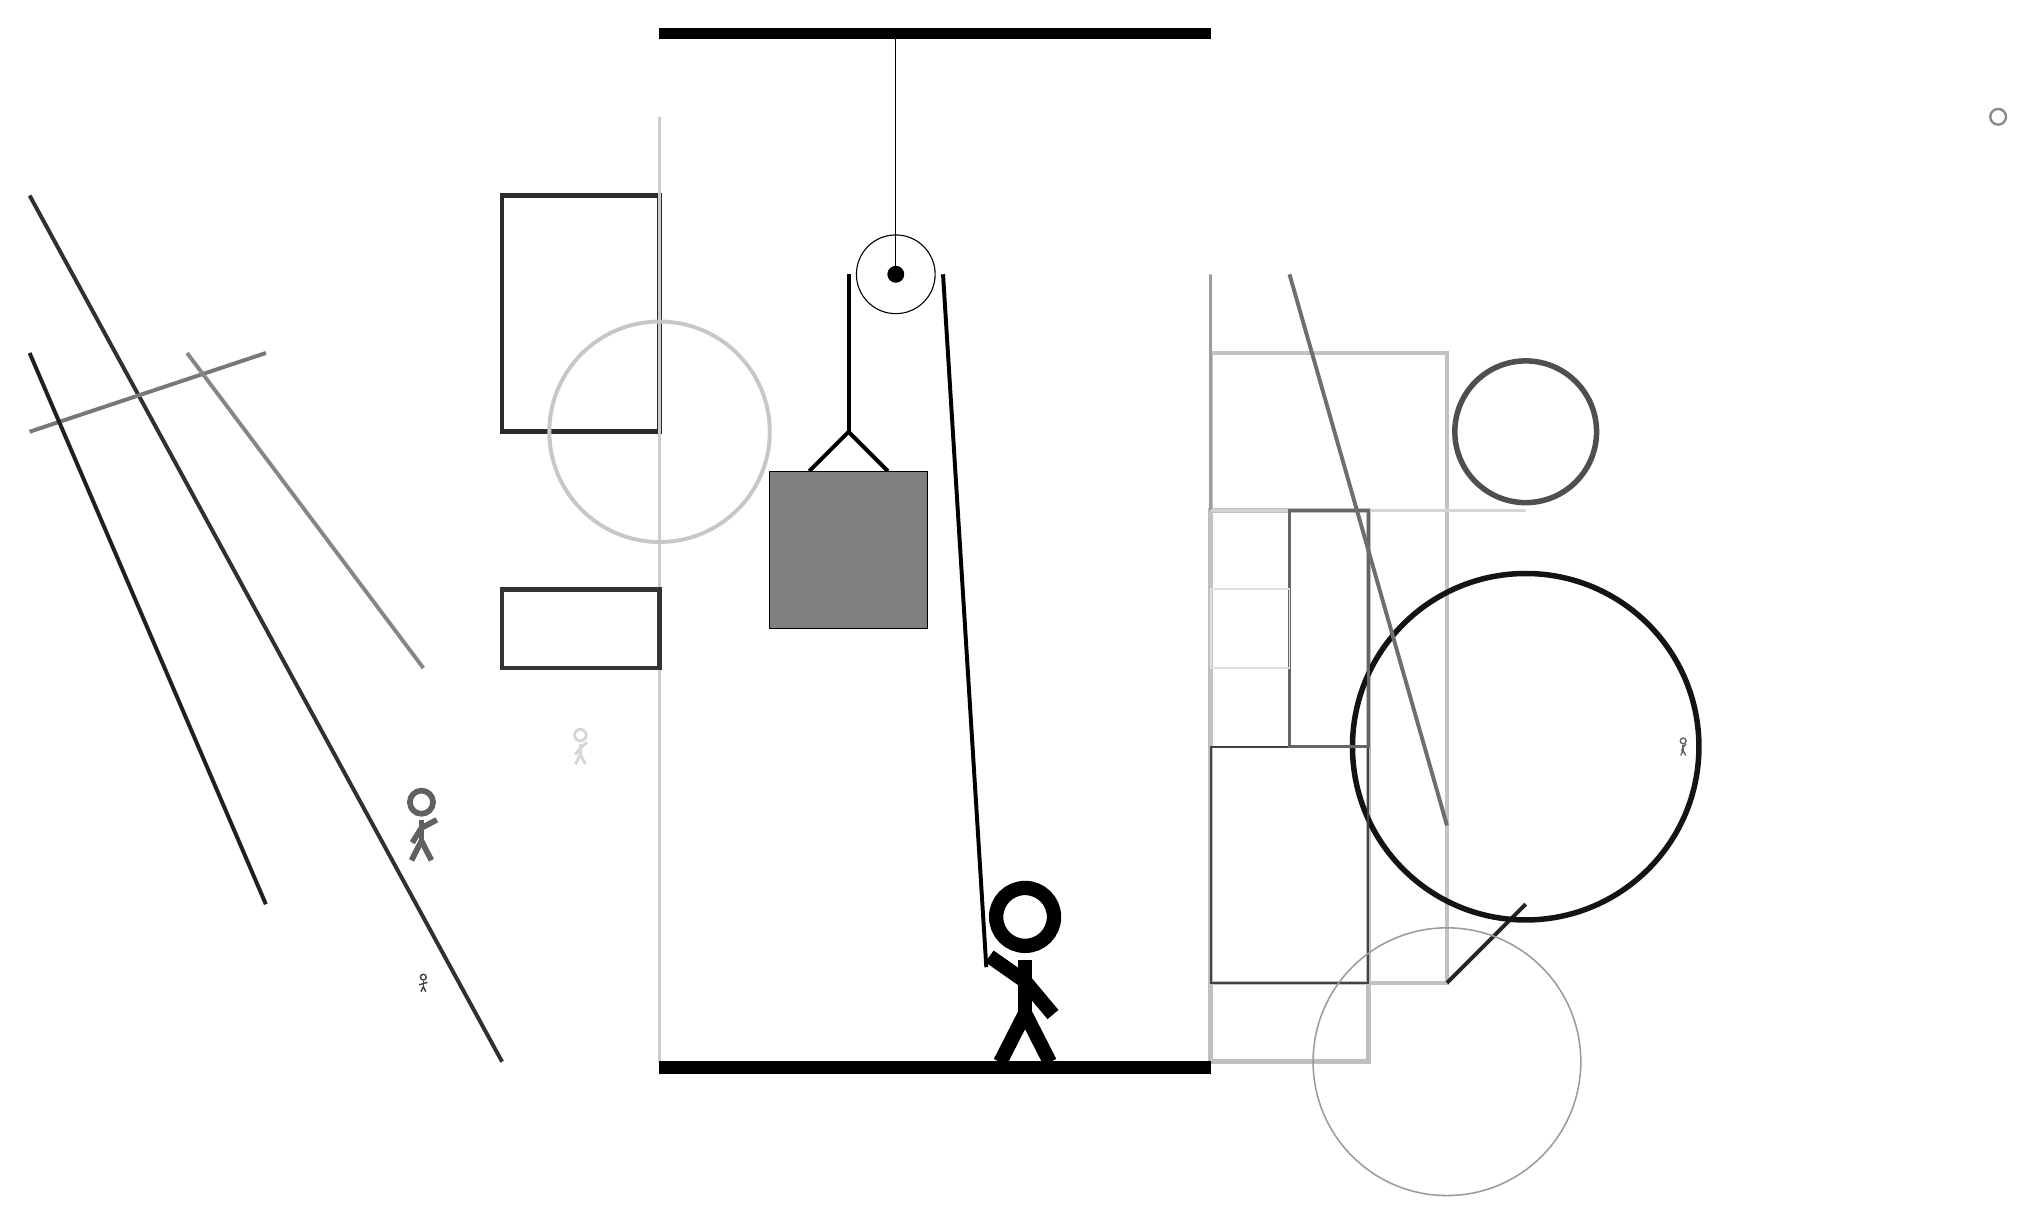
\begin{tikzpicture}
		%%%%% START %%%%%
		
		\draw[fill=black] (-2, 10) rectangle (5, 10.125);
		
		\draw (1, 7) circle (0.5);
		\draw[fill=black] (1, 7) circle (0.1);
		\draw (1, 10) -- (1, 7);
		
		\node[line width=0.2mm, color=black!16] at (-3, 1) {\Strichmaxerl[2][52][40]};
		
		\draw[line width=0.5mm, color=black!81](-4, -3) -- (-10, 8);
		\draw[line width=0.6mm, color=black!25] (7, -3) rectangle (5, 4);
		\draw[line width=0.5mm, color=black!24] (5, 6) rectangle (8, -2);
		\draw[line width=0.5mm, color=black!53](-7, 6) -- (-10, 5);
		\draw[line width=0.4mm, color=black!39] (5, 7) rectangle (5, 4);
		\draw[line width=0.4mm, color=black!17] (5, 4) rectangle (9, 4);
		
		\draw[line width=0.5mm, color=black!86](9, -1) -- (8, -2);
		\draw [line width=0.7mm, color=black!92](9, 1) circle (2.2);
		\node[line width=0.6mm, color=black!62] at (-5, 0) {\Strichmaxerl[4][58][28]};
		\draw[line width=0.2mm, color=black!74] (7, 1) rectangle (5, -2);
		\draw[line width=0.4mm, color=black!60] (6, 1) rectangle (7, 4);
		\draw[line width=0.6mm, color=black!83] (-2, 8) rectangle (-4, 5);
		\draw[line width=0.5mm, color=black!88](-7, -1) -- (-10, 6);
		\node[line width=0.5mm, color=black!61] at (11, 1) {\Strichmaxerl[1][66][52]};
		\draw[line width=0.2mm, color=black!12] (6, 2) rectangle (5, 3);
		
		\draw[line width=0.3mm, color=black!20] (-2, 9) rectangle (-2, -3);
		\draw[line width=0.5mm, color=black!57](8, 0) -- (6, 7);
		\draw [line width=0.7mm, color=black!69](9, 5) circle (0.9);
		\draw[line width=0.5mm, color=black!47](-5, 2) -- (-8, 6);
		\draw [line width=0.2mm, color=black!39](8, -3) circle (1.7);
		\draw [line width=0.5mm, color=black!22](-2, 5) circle (1.4);
		\draw [line width=0.3mm, color=black!46](15, 9) circle (0.1);
		\draw[line width=0.6mm, color=black!80] (-2, 2) rectangle (-4, 3);
		\node[line width=0.4mm, color=black!75] at (-5, -2) {\Strichmaxerl[1][17][17]};
		
		\draw[line width=0.5mm] (-0.1, 4.5) -- (0.4, 5.0) -- (0.9, 4.5);
		\draw[fill=black!50] (-0.6, 4.5) rectangle (1.4, 2.5);
		
		\draw[line width=0.5mm] (0.4, 7) -- (0.4, 5.0);
		\centerarc[line width=0.5mm](1, 7)(0:180:0.6);
		\draw[line width=0.5mm](1.6, 7) -- (2.15, -1.8);
		
		\node at (2.6, -1.9) {\Strichmaxerl[10][-35][-50]};
		
		\draw[fill=black] (-2, -3) rectangle (5, -3.15);
		
		%%%%% END %%%%%
	\end{tikzpicture}
\end{document}